\PassOptionsToPackage{russian,english,main=russian}{babel}
\documentclass{superfri}
\usepackage[T2A]{fontenc}
\usepackage[utf8]{inputenc}
\usepackage{amsmath}
\usepackage{amssymb}
\usepackage{amsthm}
\usepackage{mathrsfs}
\usepackage{booktabs}
\usepackage{multirow}
\usepackage{makecell}
\usepackage{float}
\usepackage{algorithm}
\usepackage{algpseudocode}
\usepackage[normalem]{ulem}
\usepackage{graphicx}
\usepackage{lmodern}
\usepackage[hidelinks]{hyperref}

\begin{document}

\author{D.\,A.~Grigoriev\footnote{\label{msu}Lomonosov Moscow State University, Moscow Center for Fundamental and Applied Mathematics, \\ Moscow, Russian Federation}\footnote{E-mail: dagrig14@yandex.ru} \and D.\,V.~Khudiakov\footnoteref{msu}\footnote{E-mail: hydikovv17914@gmail.com} \and D.\,I.~Chernyshev\footnoteref{msu}\footnote{E-mail: chdanorbis@yandex.ru}}

\title{Literature summarization with large language models}

\maketitle{}

\begin{abstract}
The work is dedicated to automatic summarization of Russian literary fiction.
An open corpus RuBookSum (600+ “book-summary” pairs) was compiled based on texts from LibRuSec and user-generated summaries from <<Народный Брифли>>.
Four approaches to summarization are examined: the baseline hierarchical method and the “blueprint” (Text-Blueprint) approach, 
which builds an outline in the form of question-answer pairs, as well as two new methods proposed in this work: 
a hierarchical method with node filtering based on cosine similarity of embeddings, 
and a modification of the blueprint approach with question clustering using the KMeans algorithm.
The best quality is achieved by Qwen3-235B-A22B in the blueprint method, 
while the hierarchical method with filtering provides the best balance between generation time and quality.
\keywords{LLM, summarization, literature, books, brief retelling}
\end{abstract}



% ================= ВВЕДЕНИЕ =================
\section*{Introduction}
Automatic text summarization is one of the key tasks in natural language processing. The goal is to create an informative summary of the source text while preserving its main meaning.
In recent years, with the advent of large language models (LLMs), interest in automating summarization has increased across many genres, including fiction.
Unlike scientific, news, or technical texts, fiction is characterized by high stylistic and semantic complexity.
Non-linear storytelling, imagery, metaphor, and stylistic devices make short synopsis writing especially challenging.
The limited context window of modern models further complicates processing long works.

At present moment there are not many datasets focusing specifically on summarizing fiction, and the key open datasets concentrate on non-Russian material.
BookSum \cite{BookSum} is one of the first and best-known English-language datasets for abstractive summarization of narrative works. 
It contains books, plays, and short stories paired with summaries of varying granularity (paragraph level, chapter level, book level).
Echoes from Alexandria \cite{alexandria} is a multilingual corpus of fiction, including five languages: English, German, French, Italian, and Spanish.
FABLES \cite{fables} is a hand-curated corpus designed to evaluate factual faithfulness of summaries for book-length fiction.
It includes 3,158 claims extracted from LLM-generated summaries for 26 books.
Each claim is evaluated across model outputs by experts.
According to FABLES, even advanced models (e.g., Claude) commit 20–30\% factual errors, including distorted
causal relations, incorrect characterization of protagonists, and overemphasis on minor details,
judged by three criteria: agreement with original events, logical correctness, and absence of distortions.

In theory, automatic summarization can be performed in two main ways: extractive (selecting key text fragments) and abstractive (generating new text based on the source).
For prose, abstractive summarization is typically chosen:
key meanings and plot links are distributed throughout the text, so extractive sentence selection yields a fragmented,
stylistically uneven result and does not reconstruct the plot, therefore abstractive approach was chosen.

The topic is motivated by the growing need for tools capable of automatically producing concise, informative, and stylistically appropriate synopses for works of fiction.
The goal of this work is to provide such tools, thus, following is proposed:
\begin{enumerate}
  \item New Russian-language dataset that includes literary works and their synopses;
  \item New summarization methods that offer alternatives to existing ones and substantially reduce the time required to produce a short synopsis of a book.
\end{enumerate}

Code and data are publicly available\footnote{\label{git}\url{https://github.com/Nejimaki-Tori/BookSum}}.

% ================= НАБОР ДАННЫХ =================

\section{Dataset}
At the start of the study, there were no open and representative corpora designed specifically for summarizing fiction in Russian.
To run experiments and evaluate different approaches, we created our own corpus consisting of works of fiction and corresponding short synopses.
As the source of synopses we used the “Narodny Briefly” platform \cite{Briefly} where users publish short summaries of literary works.

The synopses are user-generated texts based on the original works. They vary in length—from a few sentences to several paragraphs—and in style: some reproduce key phrases verbatim, 
while others use freer narration. Some cover the whole work, others split content by chapter.
Usually they contain the main facts and conclusions from the source text, but may include the author’s commentary.

The book texts were selected from the LibRuSec electronic library \cite{librusec}, one of the largest Russian-language fiction resources.
Works were selected for which a synopsis existed on chosen source\cite{Briefly}. Each text underwent automatic preprocessing: meta-information (e.g., titles, chapter descriptions, technical inserts) was removed,
then the text was formatted into a unified, standardized form suitable for use with models.

To better link books with their synopses, semantic similarity was used: the author name text from Briefly \cite{Briefly} and from LibRuSec \cite{librusec} was embedded via SentenceTransformer
with the model\footnote{\label{encoder}\url{https://huggingface.co/deepvk/USER-bge-m3}}
and compared using cosine similarity.

\tab{tab:dataset_info}{Dataset overview}{
\begin{tabular}{l|cccc}
\hline
\textbf{Dataset} & \makecell{Number of \\ documents} & \makecell{Avg. document \\ length \\ (\# words)} & \makecell{Avg. summary \\ length \\ (\# words)} & \makecell{Compression ratio \\ (summary length \\/ text length)} \\
\hline
\textbf{RuBookSum}  & 634 & 35052.64 & 700.77 & 8.43\% \\
\hline
BookSum    & 405 & 112885.15 & 1167.20 & 0.79\% \\
Gazeta     & 60964 & 632.77 & 41.94 & 6.99\% \\
\hline
\end{tabular}
}

The synopses were automatically cleaned of HTML tags, comments, and service markers using LLM Meta-\allowbreak Llama 3-\allowbreak 70B-\allowbreak Instruct.
Then LibRuSec was searched and a collection of “book text – synopsis” pairs was formed.
\\The resulting corpus includes:
\begin{itemize}
  \item 600+ cleaned user synopses from “Narodny Briefly” \cite{Briefly};
  \item 40+ different genres;
  \item source works from the LibRuSec electronic library \cite{librusec}.
\end{itemize}
\begin{figure}[!htbp]
    \centering
    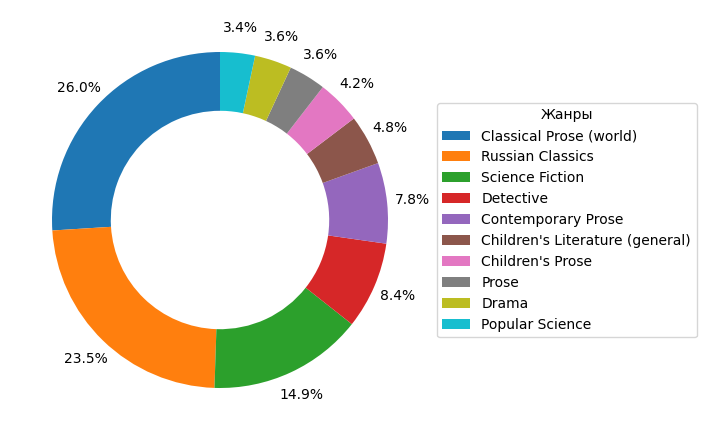
\includegraphics[width=0.8\linewidth]{figures/genres_pie.png}
    \caption{Distribution of texts by genres (top 10 genres)}
    \label{fig:genres}
\end{figure}
Figure \ref{fig:genres} shows the genre distribution in the collection. Table \tabref{tab:dataset_info} gives dataset statistics versus analogs.

% ================= МЕТОДОЛОГИЯ =================
\section{Методология}
\subsection{Базовые и модифицированные стратегии.}

\subsubsection{Иерархический метод. (Algorithm 1)}
Суть этого метода \cite{hierarchical} заключается в том, что текст разбивается на фрагменты (чанки), для каждого из
которых отдельно генерируется локальный реферат. 
Эти фрагменты затем объединяются в группы, и из полученных рефератов снова формируется краткое содержание
следующего уровня. Последний уровень представляет собой итоговый реферат всего произведения.

\subsubsection{Иерархический метод с фильтрацией узлов. (Algorithm 2)}
Классический иерархический метод строит итоговый реферат путём многослойного объединения промежуточных рефератов, полученных из отдельных фрагментов текста. 
Однако в литературных произведениях часто встречаются фрагменты, которые не оказывают большого влияния на развитие сюжета и содержат множество избыточных
повторов и второстепенной информации. Эти фрагменты при генерации итогового реферата могут снижать её информативность, а в некоторых случаях даже мешать модели на этапе реферирования отдельных фрагментов.

Чтобы решить эту проблему, в метод была имплементирована фильтрация узлов по семантической близости. 
Для исключения малоинформативных или дублирующих фрагментов на каждом уровне иерархии выполняется глобальная проверка семантической близости между всеми промежуточными рефератами. 
Фрагменты, близкие по косинусной мере с предыдущими, считаются избыточными и не используются при составлении реферата на текущем уровне.
Эмбеддинги получаются с помощью SentenceTransformer (модель USER-bge-m3) и при вычислении на GPU обеспечивается высокая скорость обработки.
Эта модификация направлена на ускорение генерации за счет удаления потенциально излишних частей информации, что повышает плотность полезной информации в итоговых рефератах. 

\noindent
\begin{minipage}[t]{0.49\textwidth}
  \begin{algorithm}[H]
  \caption{Иерархический метод}
    \begin{algorithmic}
      \Require $W$ - контекстное окно модели, $D$ - входной текст, длиной $L \gg W$, $p_\theta$ - модель, $C$ - длина чанка
      \State Разбить $D$ на чанки $c_1\dots c_{\lceil \frac{L}{C} \rceil}$
      \For{$c_i=c_1\dots c_{\lceil \frac{L}{C} \rceil}$}
        \State $S_0 \gets SummarizeChunk(p_\theta, c_i)$\
      \EndFor
      \Repeat
        \State $Groups \gets GroupSummaries(S_l)$
        \State $\ell \gets \ell + 1$
        \For{$g \in Groups$}
          \State $S_l \gets \{MergeGroup(p_\theta,g)\}$
        \EndFor
      \Until{$|S_l|=1$}
      \State \Return $S_l[1]$
    \end{algorithmic}
  \end{algorithm}
\end{minipage}\hfill
\begin{minipage}[t]{0.49\textwidth}
  \begin{algorithm}[H]
    \caption{Иерархический метод с фильтрацией}
    \begin{algorithmic}
      \Require $W$ - контекстное окно модели, $D$ - входной текст, длиной $L \gg W$, $p_\theta$ - модель, $\theta$ - порог сходства, $C$ - длина чанка
      \State Разбить $D$ на чанки $c_1\dots c_{\lceil \frac{L}{C} \rceil}$
      \State $S_0 \gets \{c_1\dots c_{\lceil \frac{L}{C} \rceil}\}$
      \Repeat
        \For{$s_i \in S_l$}
          \State $e_i \gets Encoder(s_i)$
          \State $M_{ij} \gets \dfrac{\mathbf{e}_i\cdot \mathbf{e}_j}{\|\mathbf{e}_i\|\,\|\mathbf{e}_j\|}$\Comment{Матрица эмбеддингов}
          \State{Вычисляется максимальное сходство}
        \State{с предыдущими рефератами.}
          \State $m_j=\max_{i<j} M_{ji}$
          \State $S_l \gets \{s_i \mid m_i < \theta$ \textbf{ or } $i = 0 \}$ \Comment{Фильтрация}
        \EndFor
        \State $Groups \gets GroupSummaries(S_l)$
        \State $\ell \gets \ell + 1$
        \For{$g \in Groups$}
          \State $S_l \gets \{MergeGroup(p_\theta,g)\}$
        \EndFor
      \Until{$|S_l|=1$}
      \State \Return $S_l[1]$
    \end{algorithmic}
  \end{algorithm}
\end{minipage}

\vspace{0.4em}
\subsubsection{«Чертёжный» метод (Text‑Blueprint). (Algorithm 3)}
Данный метод \cite{blueprint} по сути является модификацией иерархического и ориентирован на построение промежуточного
плана реферата перед генерацией текста. 
План формируется в виде набора вопросно-ответных пар, что повышает управляемость генерации и обеспечивает структурированность результата.
Сначала модель формирует список вопросов, отражающих ключевые события, темы
и персонажей текста. Далее к каждому вопросу автоматически подбирается краткий
ответ. Эта структура служит планом, по которому генерируется итоговый реферат.


\subsubsection{«Чертёжный» метод с кластеризацией вопросов. (Algorithm 4)}
Базовая реализация «чертёжного» метода предполагает генерацию вопросно-ответного
плана для каждого фрагмента текста и каждого уровня объединения рефератов. Однако при работе с художественными текстами вопросы, генерируемые для каждого чанка,
могут пересекаться и порождать противоречивые ответы,  то в свою очередь сбивает агрегацию текста моделью, делая реферат менее структурированным
и содержательно полным. К тому же, генерация плана на каждом шаге алгоритма существенно замедляет его работу и использует дополнительные мощности языковых моделей.
Для снижения числа запросов к модели и повышения структурности, была добавлена кластеризация вопросов с использованием SentenceTransformers и алгоритма K-means.

\noindent
\begin{minipage}[t]{0.49\textwidth}
  \begin{algorithm}[H]
    \caption{<<Чертежный>> метод}
    \begin{algorithmic}
      \Require $W$ - контекстное окно модели, $D$ - входной текст, длиной $L \gg W$, $p_\theta$ - модель, $C$ - длина чанка, $R$ - ограничение по длине
      \State Разбить $D$ на чанки $c_1\dots c_{\lceil \frac{L}{C} \rceil}$
      \For{$c_i=c_1\dots c_{\lceil \frac{L}{C} \rceil}$}
        \State $b_i \gets GenerateBlueprint(p_\theta, c_i)$\
        \State $S_0 \gets \{SummarizeWithBp(p_\theta, b_i, c_i)\}$\
      \EndFor
      \Repeat \Comment{Объединение рефератов}
        \State $Groups \gets GroupSummaries(S_l)$
        \State $\ell \gets \ell + 1$
        \For{$g \in Groups$}
          \If{$Length(g) > R$}
            \State $b_i \gets GenerateBlueprint(p_\theta, g)$\
            \State $S_l \gets \{SummarizeWithBp(p_\theta, b_i, g)\}$\
          \Else
            \State $S_l \gets \{g\}$\
          \EndIf
        \EndFor
      \Until{$|S_l|=1$}
      \State \Return $S_l[1]$
    \end{algorithmic}
  \end{algorithm}
\end{minipage}\hfill
\begin{minipage}[t]{0.49\textwidth}
  \begin{algorithm}[H]
  \caption{<<Чертежный>> метод с кластеризацией}
      \begin{algorithmic}
        \Require $W$ - контекстное окно модели, $D$ - входной текст, длиной $L \gg W$, $p_\theta$ - модель, $C$ - длина чанка, $R$ - ограничение по длине
        \State Разбить $D$ на чанки $c_1\dots c_{\lceil \frac{L}{C} \rceil}$
        \For{$c_i=c_1\dots c_{\lceil \frac{L}{C} \rceil}$}
          \State $b_i \gets GenerateBlueprint(p_\theta, c_i)$
          \State $Q \gets \{ExtractQuestions(p_\theta, b_i)\}$
        \EndFor
        \For{$q_i \in Q$}
          \State $E \gets \{Encoder(q_i)\}$
          \State $K \gets KMeans(E)$
          \For{$k_i \in K$}
            \State $q_i \gets Generalize(p_\theta, k_i)$
            \State $Q \gets \{q_i\}$ \Comment{Собирается общий план}
          \EndFor
          \For{$c_i=c_1\dots c_{\lceil \frac{L}{C} \rceil}$}
            \State $S_0 \gets \{SumWithBp(p_\theta, b_i, c_i)\}$\
          \EndFor
        \EndFor
        \State \textbf{Объединение рефератов} аналогично <<Чертежному методу>> с тем отличием что здесь в качестве чертежа используется один глобальный план Q
      \end{algorithmic}
  \end{algorithm}
\end{minipage}

Такой подход позволяет уменьшить число обращений к LLM, что позволяет ускорить скорость генераций, как будет показано в таблице \ref{tab:results_models}.

% ================= МЕТРИКИ =================

\section{Метрики}

Для объективного сравнения описанных подходов и моделей в задаче реферирования художественных текстов использовались четыре группы метрик.

\textbf{ROUGE-L} \cite{rouge} - основана на длине наибольшей общей подпоследовательности (LCS) между сгенерированным рефератом $S$ и эталонным $R$.
Вычисляется по формуле \eqref{rouge} с использованием формул \eqref{r_p} и \eqref{r_r}:
\begin{equation}\label{r_p}
  \text{Precision} = \frac{\mathrm{LCS}(S,R)}{|S|},\quad
\end{equation}
\begin{equation}\label{r_r}
  \text{Recall} = \frac{\mathrm{LCS}(S,R)}{|R|}
\end{equation}
\begin{equation}\label{rouge}
  \text{ROUGE‑L} = \frac{2\;\text{Precision}\;\cdot\;\text{Recall}}{\text{Precision} + \text{Recall}}
\end{equation}

\textbf{BERTScore} \cite{bertscore} - семантическое качество на уровне токенов. Для каждой пары токенов предсказания и эталона вычисляется косинусное сходство их эмбеддингов в модели USER‑bge‑m3. Затем:
\begin{equation}\label{precision}
P = \frac{1}{|S|}\sum_{t\in S}\max_{u\in R}\!\mathrm{sim}(e_t, e_u),\quad
\end{equation}

\begin{equation}\label{recall}
R = \frac{1}{|R|}\sum_{u\in R}\max_{t\in S}\!\mathrm{sim}(e_u, e_t)\\
\end{equation}

\begin{equation}\label{f}
\text{BERTScore} = \frac{2\,P\,R}{P+R}
\end{equation}

В формулах  \eqref{precision}, \eqref{recall} и \eqref{f} \(S\) - эталонный текст, \(R\) - сгенерированный; каждое предложение кодируется эмбеддингом модели USER‑bge‑m3, 
после чего вычисляется косинусное сходство.  

\textbf{Полнота покрытия ключевых вопросов (Coverage)} - доля заранее сгенерированных по эталонному тексту вопросов с помощью модели Qwen3-\allowbreak 235B-\allowbreak A22B \cite{qwen3},
на которые модель «отвечает» в реферате:
\begin{equation}\label{coverage}
  \text{Coverage} = \frac{\#\{q_i\colon P(\text{“да”}\mid q_i,S)\!>\!0.75\}}{N}
\end{equation}
В формуле \eqref{coverage} $N$ - общее число вопросов, а $P(\text{“да”}\mid q_i,S)$ - вероятность наличия ответа на вопрос $q_i$ в тексте $S$, 
полученная с помощью LLM (Qwen3-\allowbreak 235B-\allowbreak A22B \cite{qwen3}).

\textbf{Совпадение ответов (AnswerSimilarity)} - среднее семантическое сходство между сгенерированными ответами $a_i^{\text{pred}}$ и эталонными $a_i^{\text{ref}}$ на те же ключевые вопросы:
\begin{equation}\label{sims}
  \text{AnswerSimilarity} = \frac{1}{N}\sum_{i=1}^N \mathrm{sim}\bigl(a_i^{\text{pred}},\,a_i^{\text{ref}}\bigr)
\end{equation}
В формуле \eqref{sims} $\mathrm{sim}$ - косинусное сходство эмбеддингов, полученных через USER‑bge‑m3.


Использование нескольких метрик, учитывающих как поверхностное совпадение текста, так и глубокое семантическое сходство (BERTScore, AnswerSimilarity), 
а также степень охвата заранее заданных вопросов (Coverage), обеспечивает всестороннюю и устойчивую оценку качества рефератов.

\section{Параметры экспериментов}

Все представленные в работе измерения выполнены на тестовой части датасета, 
отобранных так, чтобы исходные тексты не превышали по длине 800\,000 символов. 
Для всех методов генерируемые рефераты ограничивались максимумом в 500 слов.

Текст на вход разбивался на чанки фиксированного размера в 2000 токенов. 
Токенизация выполнялась с помощью \texttt{AutoTokenizer} модели \texttt{DeepPavlov/rubert-base-cased} в стандартном режиме.
Для воспроизводимости всех случайных процедур использовался фиксированный seed ($random\_seed = 42$).

В \textbf{иерархическом методе с фильтрацией узлов} для оценки избыточности промежуточных рефератов на каждом уровне вычислялась матрица косинусных сходств между их эмбеддингами.
Порог схожести был установлен равным $\theta=0.85$: если для реферата $S_j$ существует предыдущий $S_i$ с косинусным сходством выше этого порога, 
то $S_j$ отбрасывается как избыточный. Такой выбор порога обеспечивает компромисс между сохранением значимой информации и устранением дублирования, 
что эмпирически привело к заметному уменьшению объёма промежуточных представлений без существенной деградации качества.

В \textbf{чертёжном методе с кластеризацией вопросов} количество кластеров для K-means выбирается по эвристике, подобранной эмпирически, представленной в формуле \eqref{num_cl}:
\begin{equation}\label{num_cl}
  n_{\text{clusters}} = \max\!\left(2,\; \left\lceil \sqrt{N_{\text{questions}}} \right\rceil\right)
\end{equation}

где $N_{\text{questions}}$ - общее число сгенерированных вопросов по всем чанкам до кластеризации. 
Гарантируется минимум в два кластера, что позволяет даже при небольших наборах вопросов получать структурированное чертёжное представление.

Временные показатели измерялись как среднее значение (в секундах) времени генерации одной книги по каждому методу для 100 книг. 
В случае всех четырех методов учитывалось суммарное время всех этапов (включая генерацию промежуточных рефератов / планов, фильтрацию и финальную агрегацию).

% ================= РЕЗУЛЬТАТЫ =================

\section{Результаты}

\subsection{Используемые модели.}
В экспериментах использовались следующие большие языковые модели: 
RuadaptQwen2.5-\allowbreak 7B-\allowbreak Lite-\allowbreak Beta \cite{ruadapt}, 
RuadaptQwen3-\allowbreak 32BInstruct-v2 \cite{ruadapt}, 
DeepSeek V3 \cite{deepseek}, 
Qwen3-\allowbreak 235B-\allowbreak A22B \cite{qwen3}, 
tpro \cite{tpro} и yagpt5lite \cite{yagpt}.

\tab{tab:results_models}{Результаты по методам и моделям}{
\centering
\small
\setlength{\tabcolsep}{4pt}
\begin{tabular}{ll|c|c|c|c}
\toprule
Модель & Метрики &
\makecell{Иерархический} &
\makecell{Чертежный} &
\makecell{Иерархический \\ с фильтрацией} &
\makecell{Чертежный \\ с кластеризацией} \\
\hline
\multirow{5}{*}{DeepSeek V3}
 & bertscore  & \uline{60.0 ± 3.1} & 58.0 ± 4.0 & 60.0 ± 2.9 & 58.4 ± 3.6 \\
 & rouge-l    & 13.7 ± 3.9 & 12.6 ± 4.6 & 13.5 ± 3.7 & 11.2 ± 3.9 \\
 & coverage   & \uline{\textbf{53.57 ± 21.66}} & 40.19 ± 23.68 & \uline{\textbf{45.00 ± 23.03}} & \uline{\textbf{34.68 ± 23.77}} \\
 & similarity & \uline{42.38 ± 17.73} & 32.31 ± 19.33 & 35.64 ± 18.88 & \uline{27.76 ± 19.75} \\
 & time       & 196.77 ± 187.85 & 315.67 ± 321.89 & 147.21 ± 146.4 & 132.60 ± 197.25 \\
\multirow{5}{*}{Qwen3-235B-A22B}
 & bertscore  & 61.2 ± 3.0 & \uline{61.6 ± 3.3} & \uline{60.9 ± 2.7} & \uline{59.3 ± 3.4} \\
 & rouge-l    & \uline{14.9 ± 4.0} & \uline{15.8 ± 4.5} & \uline{14.8 ± 3.7} & \uline{12.2 ± 3.6} \\
 & coverage   & 52.48 ± 20.79 & \uline{\textbf{54.78 ± 21.16}} & 44.54 ± 23.03 & 30.19 ± 21.96 \\
 & similarity & 41.68 ± 17.18 & \uline{43.99 ± 17.54} & \uline{35.67 ± 18.87} & 24.10 ± 17.62 \\
 & time       & 103.49 ± 97.30 & 230.35 ± 271.03 & 83.06 ± 102.05 & 158.30 ± 196.35 \\
 \hline
\multirow{5}{*}{\makecell{RuadaptQwen3-32B\\Instruct-v2}}
 & bertscore  & 57.3 ± 2.9 & 58.9 ± 3.6 & 57.7 ± 3.3 & 55.3 ± 3.3 \\
 & rouge-l    & 11.0 ± 2.4 & 10.6 ± 3.2 & 10.7 ± 2.4 & 7.8 ± 2.1 \\
 & coverage   & 33.12 ± 21.50 & 33.18 ± 22.83 & 32.19 ± 22.52 & 17.72 ± 15.23 \\
 & similarity & 25.25 ± 16.94 & 26.21 ± 18.22 & 24.82 ± 17.74 & 13.97 ± 12.39 \\
 & time       & 218.30 ± 195.16 & 379.24 ± 500.40 & 166.79 ± 164.61 & 286.35 ± 395.97 \\
\multirow{5}{*}{tpro}
 & bertscore  & \uline{59.4 ± 3.0} & \uline{59.0 ± 4.9} & \uline{59.5 ± 3.3} & \uline{58.2 ± 3.7} \\
 & rouge-l    & \uline{13.8 ± 3.1} & \uline{14.7 ± 4.9} & \uline{13.5 ± 3.0} & \uline{11.8 ± 3.9} \\
 & coverage   & \uline{40.27 ± 20.23} & \uline{40.83 ± 22.42} & \uline{37.13 ± 20.72} & \uline{26.03 ± 18.44} \\
 & similarity & \uline{31.77 ± 16.63} & \uline{32.60 ± 18.57} & \uline{29.44 ± 16.83} & \uline{20.83 ± 15.26} \\
 & time       & 367.32 ± 324.49 & 592.39 ± 772.19 & 267.73 ± 253.34 & 247.59 ± 361.20 \\
 \hline
\multirow{5}{*}{\makecell{RuadaptQwen2.5-7B\\Lite-Beta}}
 & bertscore  & 55.4 ± 2.9 & 56.1 ± 4.9 & 55.8 ± 2.9 & 54.0 ± 4.0 \\
 & rouge-l    & 8.6 ± 2.5 & 10.1 ± 3.9 & 8.7 ± 2.5 & 7.7 ± 2.8 \\
 & coverage   & 19.66 ± 17.77 & 24.94 ± 21.08 & 20.31 ± 17.95 & 15.51 ± 14.83 \\
 & similarity & 15.16 ± 14.11 & 20.03 ± 17.50 & 15.94 ± 14.39 & 12.23 ± 12.30 \\
 & time       & 68.86 ± 64.85 & 126.84 ± 145.74 & 53.59 ± 47.28 & 76.66 ± 91.78 \\
\multirow{5}{*}{yagpt5lite}
 & bertscore  & \uline{62.5 ± 3.5} & \uline{61.1 ± 3.8} & \uline{62.1 ± 3.2} & \uline{61.5 ± 3.3} \\
 & rouge-l    & \uline{16.9 ± 5.1} & \uline{15.8 ± 5.1} & \uline{16.4 ± 4.7} & \uline{14.3 ± 4.4} \\
 & coverage   & \uline{36.85 ± 19.40} & \uline{33.17 ± 21.58} & \uline{31.75 ± 20.06} & \uline{24.28 ± 16.95} \\
 & similarity & \uline{29.69 ± 16.43} & \uline{26.58 ± 18.13} & \uline{25.60 ± 16.85} & \uline{19.70 ± 14.29} \\
 & time       & 31.02 ± 28.51 & 113.34 ± 123.78 & 27.39 ± 28.05 & 42.15 ± 56.50 \\
\bottomrule
\end{tabular}
}

\subsection{Полученные результаты.}
В таблице \ref{tab:results_models} представлены сравнительные метрики качества автоматического пересказа книг разными моделями и методами обработки. Для каждой комбинации модели и метода измерялись BERTScore, ROUGEL, Answer Coverage и 
Similarity, а также время генерации (среднее) на 100 примерах, одинаковых для всех замеров. Лучше всего себя показала модель Qwen3-\allowbreak 235B-\allowbreak A22B: она продемонстрировала самые высокие показатели в покрытие вопросов и сходстве ответов.
В то же время важно отметить, что среди всех методов лучшим образом в соотношение качество и время обработки себя показывает иерархический метод с фильтрацией узлов. Он позволяет существенно ускорить время обработки (например, почти в два раза для модели DeepSeek V3), и по сравнению с 
чертежным методом, который в среднем показывал лучшие результаты, не сильно отстает по показателям. Исключением стала лишь модель Qwen3-\allowbreak 235B-\allowbreak A22B, так как она показала лучший результат среди всех моделей на базовом чертежном методе.
Эксперименты показали, что иерархический метод с фильтрацией узлов обеспечивает наилучший компромисс между скоростью и качеством генерации.

\subsection{Анализ и сравнение результатов.}
Разброс значений метрики QA можно проиллюстрировать на примере работы одной и той же модели (DeepSeek V3) в рамках иерархического метода.
В качестве иллюстрации взяты два реферата к произведениям <<И грянул гром>> и <<Кастрюк>>. 
В первом случае модель получила высокий результат, ответив на все, кроме одного вопроса; во втором
реферате содержались ответы только на два вопроса из одиннадцати, что привело к низкому показателю. На рисунке \ref{fig:refs} показаны два реферата. 
Для краткости в них выделены только основные моменты, которые
повлияли на итоговую метрику. 
Сравнение показывает возможную причину столь значительного расхождения: реферат к рассказу <<Кастрюк>> содержит большое количество лирических отступлений и художественных деталей,
из-за чего суть произведения сложно уловить и модель отвлекается от фиксации главных фактов,
тогда как в "И грянул гром" события изложены последовательно и структурировано, 
а основные элементы сюжета чётко перечислены, что существенно упрощает задачу поиска важной информации.
В текстах выделены жирным шрифтом фрагменты, которые несут в себе важную сюжетную информацию, а подчеркнутый текст - то, что можно было бы опустить.

\begin{figure}[ht!]
  \centering
  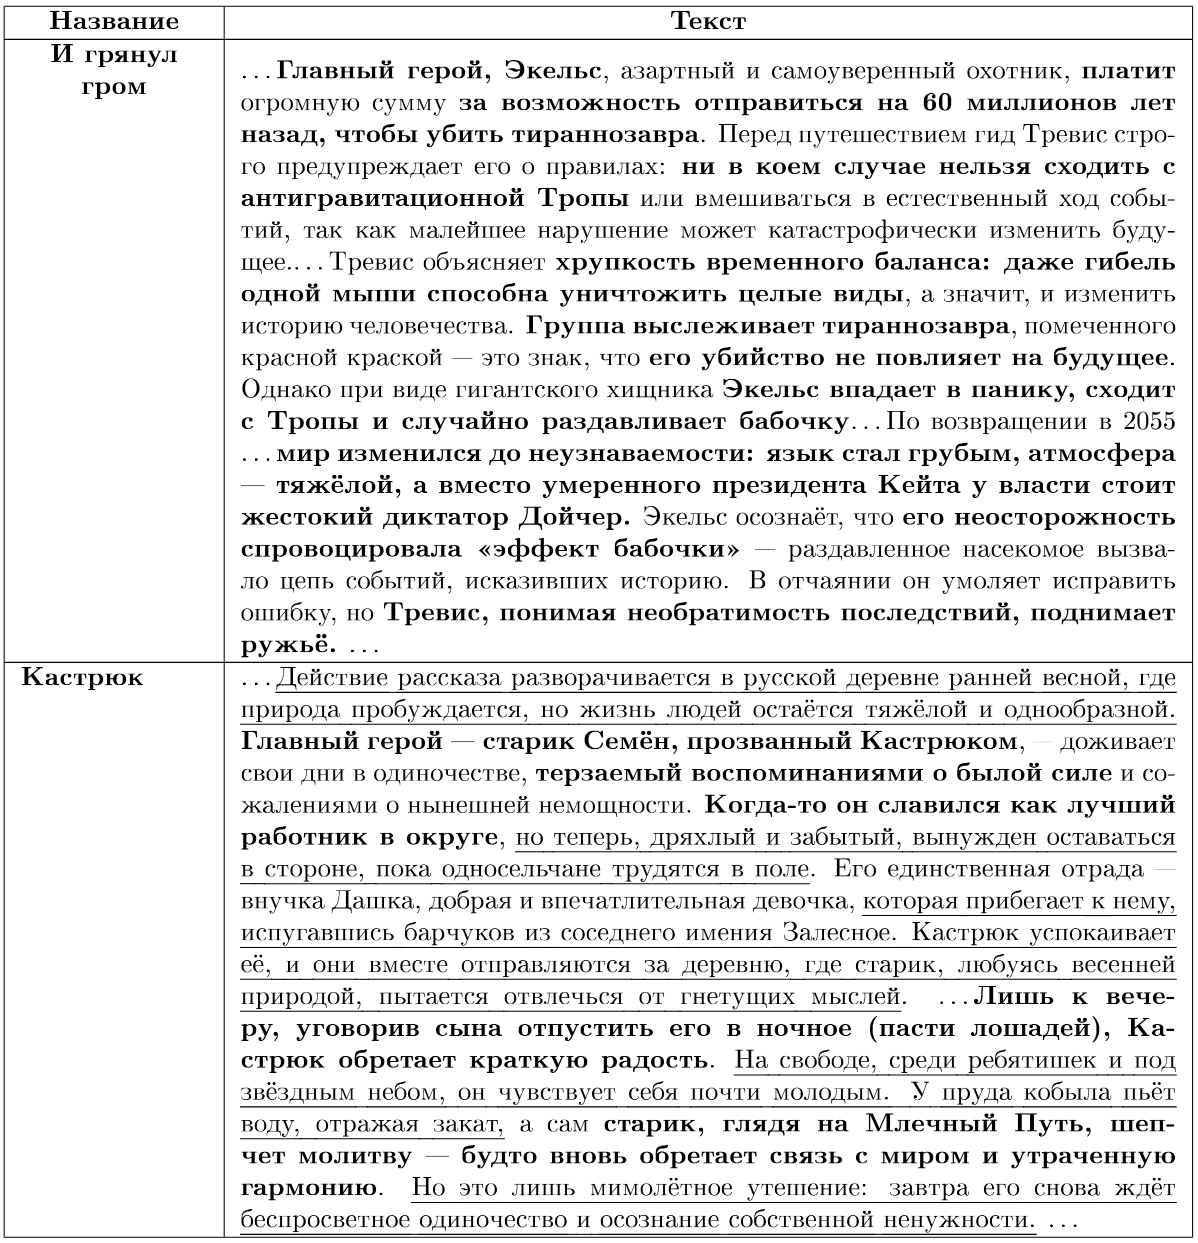
\includegraphics[width=0.9\textwidth]{figures/two_ref.png}
  \caption{Сравнение лучшего и худшего сгенерированного реферата}
  \label{fig:refs}
\end{figure}

\begin{figure}[ht!]
  \centering
  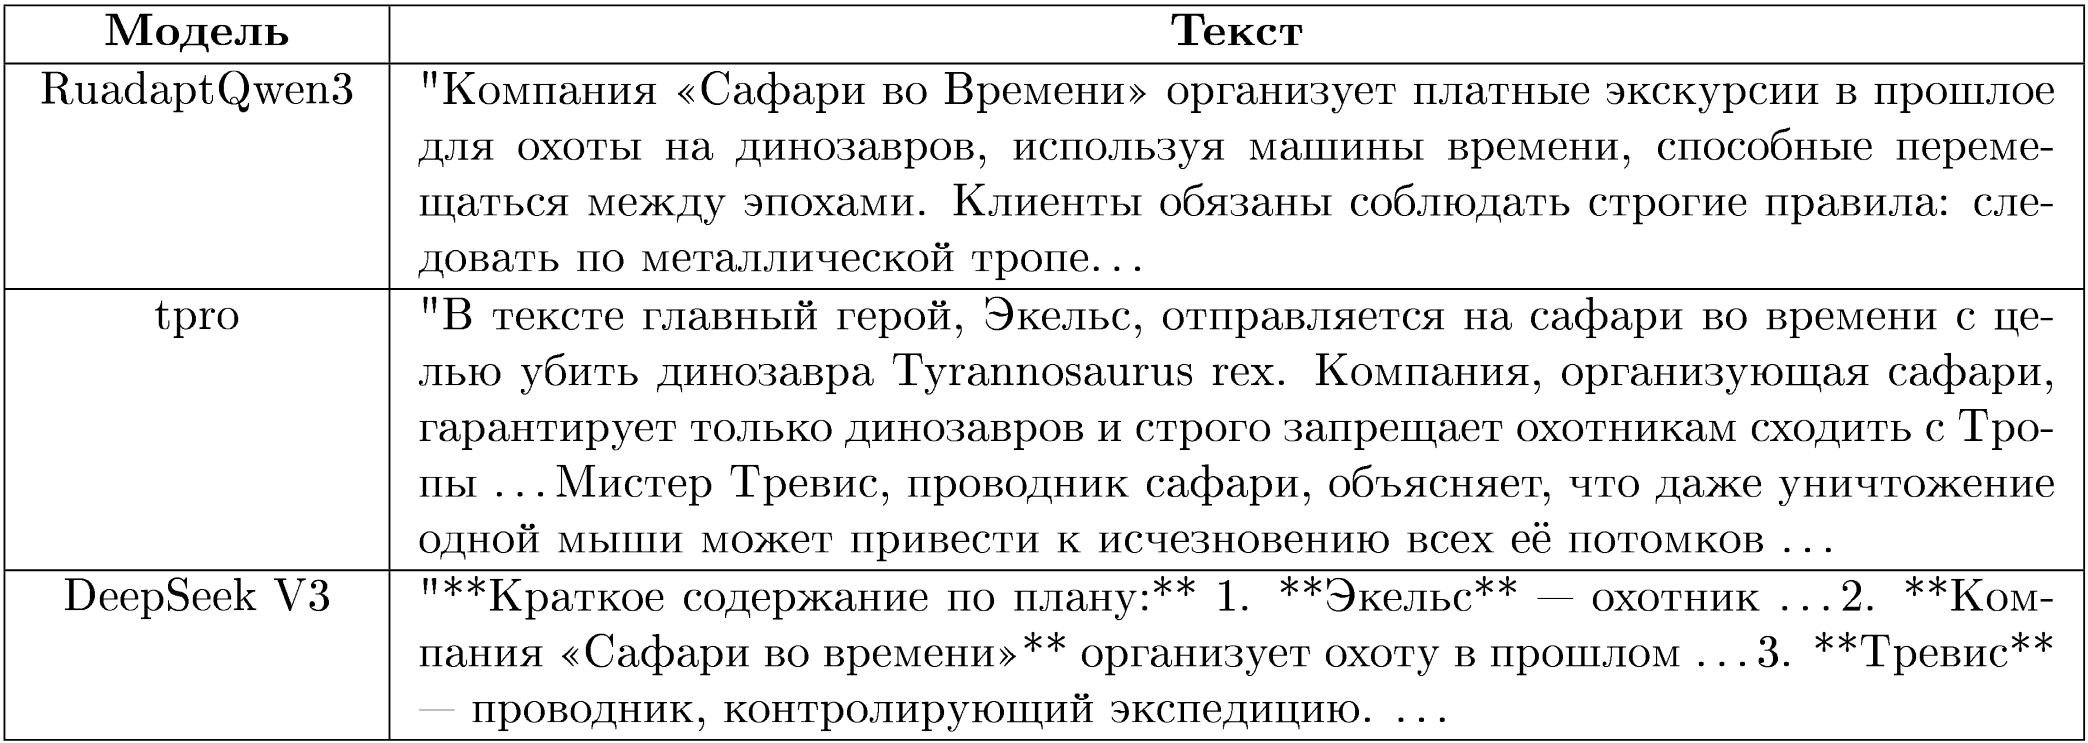
\includegraphics[width=0.9\textwidth]{figures/three_ref.png}
  \caption{Сравнение моделей при генерации рефератов по чертежному методу}
  \label{fig:bl_ref}
\end{figure}

Переходя к сравнению между моделями, можно отметить, что в целом DeepSeek V3 показывает лучшие показатели, чем модели меньшей категории, однако, если сравнивать чертежный метод, то в 30\% случаев модель 
RuadaptQwen3-\allowbreak 32B-\allowbreak Instruct-\allowbreak v2 показывает лучшие результаты, а tpro в 43\%. Для сравнения можно взять реферат по произведению <<И грянул гром>>, созданную с использованием чертежного метода, 
небольшие вырезки которой приведены на рисунке \ref{fig:bl_ref}.
В то время как реферат, созданный моделью DeepSeek V3 больше похожа на перечисление основных событий через нумерованный список,
текст у моделей RuadaptQwen3-\allowbreak 32B-\allowbreak Instruct-\allowbreak v2 и tpro является связным пересказом текста, раскрывающим все основные события сюжета.

Следует отметить, что лучшего результата удалось добиться именно чертежным методом с помощью большой модели Qwen3-\allowbreak 235B-\allowbreak A22B, 
как было показано в таблице \ref{tab:results_models}. Для сравнения качества рефератов можно взять рассказ <<Барбос и Жулька>> - в иерархическом методе
модель Qwen3-\allowbreak 235B-\allowbreak A22B посчитала, что <<Жулька>> - не собака, а лошадь. Также, например, DeepSeek V3 более строго следует шаблону чертежного метода и вместо связного текста пересказа получается нумерованный список
пунктов с ключевыми событиями и главными героями. Однако Qwen3-\allowbreak 235B-\allowbreak A22B пишет обычный текст, без списков. Таким образом, чертежный метод без модификаций позволил достичь наилучшего результата с использованием лучшей доступной моделью - 
Qwen3-\allowbreak 235B-\allowbreak A22B.

\subsection{Замеры времени.}
Проводились первоначальные замеры скорости работы методов на небольших текстах, полученные результаты в секундах (среднее по трём запускам) представлены в таблице~\tabref{tab:timing}.
Результаты подтверждают, что модификации позволяют повысить скорость генерации.

\tab{tab:timing}{Время генерации рефератов (в секундах) для текста размером 81{,}049 символов (11 чанков). Усреднено по трём запускам.}{
  \small
\begin{tabular}{lcccc}
\textbf{Модель} & \makecell{Иерархический} & \makecell{Иерархический\\с фильтрацией} & \makecell{Чертежный} & \makecell{Чертежный\\с кластеризацией} \\
\hline
DeepSeek V3                  & 237.83 & 72.42 & 292.80 & 268.75 \\
Qwen3-235B-A22B              & 113.24 & 39.45 & 215.63 & 145.20 \\
\hline
RuadaptQwen3-32BInstruct-v2  & 218.23 & 72.54 & 420.95 & 470.4 \\
tpro                         & 472.23 & 127.38 & 421.65 & 185.94 \\
\hline
RuadaptQwen2.5-7B-Lite-Beta  & 84.64 & 25.70 & 103.66 & 78.99 \\
yagpt5lite                   & 34.17 & 14.08 & 99.70 & 27.26 \\
\end{tabular}
}

Интересно отметить, что сверхкрупные модели, такие как Qwen3-235B-A22B и DeepSeek V3, продемонстрировали более высокую скорость работы, 
чем некоторые модели с размером 32B.
Ключевая причина этого заключается в использовании архитектуры MoE (Mixture of Experts):
во время генерации активна лишь ограниченная часть параметров (например, порядка 30 млрд вместо всех 600 млрд),
кроме того, такие модели, как правило, дополнительно оптимизированы для повышения производительности.

% ================= ЗАКЛЮЧЕНИЕ =================

\section*{Заключение}
В заключение, был создан первый открытый датасет, объединяющий тексты книг и рефератов к ним с открытого ресурса <<Народный Брифли>> \cite{Briefly}. 
В работе предложены два улучшенных подхода к реферированию художественных текстов с использованием LLM: иерархический с фильтрацией и чертёжный с кластеризацией. 
Иерархический метод с фильтрацией позволяет ускорить генерацию при минимальной потере качества, 
что делает этот метод пригодным для обработки длинных произведений в условиях ограниченного контекста моделей.  

Сравнительный анализ показал, что крупные модели, такие как DeepSeek~V3 и Qwen3-\allowbreak 235B-\allowbreak A22B, в большинстве случаев обеспечивают более высокое покрытие QA и 
большую полноту рефератов по сравнению с компактными моделями, особенно в иерархическом и чертёжном методах. 
Однако для некоторых типов текстов и методов (например, базовый чертёжный) более компактные модели, такие как RuadaptQwen3-\allowbreak 32B-\allowbreak Instruct-\allowbreak v2, 
могут демонстрировать конкурентоспособное качество при меньших вычислительных затратах. 
Таким образом, выбор модели следует определять исходя из баланса между доступными ресурсами, требованиями к качеству и характером обрабатываемых текстов.

\section*{Благодарности}
Исследование выполнено за счет гранта Российского научного фонда № 25-11-00191, \\https://rscf.ru/project/25-11-00191/

Работа выполнялась с использованием суперкомпьютера «МГУ-270» МГУ имени М.В. Ломоносова.
% ================= ЛИТЕРАТУРА =================



\openaccess

\bibliographystyle{superfri}
\begin{thebibliography}{99}
\bibitem{BookSum}
BOOKSUM: A Collection of Datasets for Long-form Narrative Summarization / Wojciech Kryscinski, Nazneen Rajani, Divyansh Agarwal et al. // Findings of the Association for Computational Linguistics: EMNLP 2022 / Ed. by Yoav Goldberg, Zornitsa Kozareva, Yue Zhang. - Abu Dhabi, United Arab Emirates: Association for Computational Linguistics, 2022. - . - Pp. 6536-6558. https://aclanthology.org/2022.findings-emnlp.488/.

\bibitem{alexandria}
Echoes from Alexandria: A Large Resource for Multilingual Book Summarization / Alessandro Scir`e, Simone Conia, Simone Ciciliano, Roberto Navigli // Findings of the Association for Computational Linguistics: ACL 2023 / Ed. by Anna Rogers, Jordan Boyd-Graber, Naoaki Okazaki. - Toronto, Canada: Association for Computational Linguistics, 2023. - . - Pp. 853-867. https://aclanthology.org/2023.findings-acl.54/.

\bibitem{fables}
FABLES: Evaluating faithfulness and content selection in book-length summarization \\/ Yekyung Kim, Yapei Chang, Marzena Karpinska et al. // First Conference on Language Modeling. - 2024. https://openreview.net/forum?id=YfHxQSoaWU.

\bibitem{Briefly}
\textit{Народный Брифли.}  
Электронная библиотека кратких пересказов литературных произведений.  
\url{https://wiki.briefly.ru/} (дата обращения: 30.07.2025).

\bibitem{librusec}
Библиотека художественных произведений.  
\url{https://librusec.org//} (дата обращения: 30.07.2025).

\bibitem{hierarchical} 
Wu J. et al. Recursively Summarizing Books with Human Feedback //arXiv e-prints. - 2021. - С. arXiv: 2109.10862.

\bibitem{blueprint} 
Text-Blueprint: An Interactive Platform for Plan-based Conditional Generation / \\Fantine Huot, Joshua Maynez, Shashi Narayan et al. // Proceedings of the 17th Conference of the European Chapter of the Association for Computational Linguistics:
System Demonstrations / Ed. by Danilo Croce, Luca Soldaini. - Dubrovnik, Croatia: Association for Computational Linguistics, 2023. - . - Pp. 105-116. https:
//aclanthology.org/2023.eacl-demo.13/.

\bibitem{rouge}
\textit{ROUGE.}
Lin C. Y. Rouge: A package for automatic evaluation of summaries //Text summarization branches out. - 2004. - С. 74-81.

\bibitem{bertscore}
\textit{BERTScore.}
BUCKLEY C. Evaluating Evaluation Measure Stability //ACM SIGIR 2000 Proceedings. - 2000.

\bibitem{qwen3}
\textit{Qwen3-235B.}
Yang A. et al. Qwen3 technical report //arXiv preprint arXiv:2505.09388. - 2025.

\bibitem{ruadapt}
\textit{RuadaptQwen.}
Tikhomirov M., Chernyshev D. Facilitating large language model russian adaptation with learned embedding propagation //Journal of Language and Education. - 2024. - Т. 10. - №. 4 (40). - С. 130-145.

\bibitem{deepseek}
\textit{DeepSeek V3.}
Liu A. et al. DeepSeek-V3 Technical Report //CoRR. - 2024.

\bibitem{tpro}
Т-Банк открыл доступ к собственной русскоязычной языковой модели в весовой категории 7-8 млрд параметров\\ Т-Банк URL: https://www.tbank.ru/about/news/20072024-t-bank-opened-access-its-own-russian-\\language-language-model-weight-category-of-7-8-billion-parameters/ (дата обращения: 10.05.2025).

\bibitem{yagpt}
YandexGPT 5 с режимом рассуждений // Яндекс URL: https://ya.ru/ai/gpt?ysclid=mal9jrssc8906806775 (дата обращения: 30.07.2025).

\end{thebibliography}

\end{document}
